\documentclass[a4paper]{article}

\usepackage[T1]{fontenc}
\usepackage[utf8]{inputenc}

\usepackage{mathptmx}

\usepackage{subcaption}
\usepackage[shortlabels]{enumitem}
\usepackage{amsmath,amssymb}
\usepackage{amsthm}
\usepackage{bbm}
\usepackage{graphicx}
\usepackage[colorlinks=true,naturalnames=true,plainpages=false,pdfpagelabels=true]{hyperref}
\usepackage[parfill]{parskip}

\usepackage{tikz}
\usetikzlibrary{patterns,decorations.pathmorphing,positioning}

\theoremstyle{definition}
\newtheorem{definition}{Definition}

\theoremstyle{definition}
\newtheorem{question}{Question}

\theoremstyle{definition}
\newtheorem{example}{Example}

\theoremstyle{theorem}
\newtheorem{theorem}{Theorem}

\theoremstyle{theorem}
\newtheorem{lemma}{Lemma}

\theoremstyle{theorem}
\newtheorem{exercise}{Exercise}

\theoremstyle{definition}
\newtheorem{solution}{Solution}

\newtheorem*{idea}{Proof Idea}


\title{Notes on \\ Noncommutative Geometry and Particle Physics}
\author{Popovic Milutin}
\date{Week 5: 12.03 - 19.03}

\begin{document}

\maketitle
\tableofcontents

\section{Noncommutative Geometric Spaces }
\subsection{Exercises}
\begin{exercise}
    Make the proof of the last theorem (see week4.pdf) explicit for $N=3$
\end{exercise}
\begin{solution}
    For the C* algebra we have $A=\mathbb{C}^3$
    For $H$ we have $H = (\mathbb{C}^2)^{\oplus 3} = H_2 \oplus H_2^1 \oplus H_2^2$.
    The symmetric operator $D$ acting on $H$ and the representation $\pi (a)$:
    \begin{align}
        \pi((a(1), a(2), a(3)) &=
        \begin{pmatrix}
            a(1) & 0 \\ 0 & a(2)
        \end{pmatrix} \oplus
        \begin{pmatrix}
            a(1) & 0 \\ 0 & a(3)
        \end{pmatrix} \oplus
        \begin{pmatrix}
            a(2) & 0 \\ 0 & a(2)
        \end{pmatrix} \nonumber  \\
        & =
        \begin{pmatrix}
            a(1) & 0 & 0 & 0 & 0 & 0 \\
            0    & a(2) & 0 & 0 & 0 & 0 \\
            0    & 0 & a(1) & 0 & 0 & 0 \\
            0    & 0 & 0 & a(3) & 0 & 0 \\
            0    & 0 & 0 & 0 & a(2) & 0 \\
            0    & 0 & 0 & 0 & 0 & a(3)
        \end{pmatrix} \\
        D &=
        \begin{pmatrix}
            0 & x_1 \\ x_1 & 0
        \end{pmatrix} \oplus
        \begin{pmatrix}
            0 & x_1 \\ x_1 & 0
        \end{pmatrix} \oplus
        \begin{pmatrix}
            0 & x_1 \\ x_1 & 0
        \end{pmatrix} \nonumber \\
        &=
        \begin{pmatrix}
            0   & x_1 & 0 & 0 & 0 & 0 \\
            x_1 & 0   & 0 & 0 & 0 & 0 \\
            0   & 0   & 0 & x_2 & 0 & 0 \\
            0   & 0   & x_2 & 0 & 0 & 0 \\
            0   & 0   & 0 & 0 & 0 & x_3 \\
            0   & 0   & 0 & 0 & x_3 & 0 \\
        \end{pmatrix} \\
    \end{align}
    Then the norm of the commutator would be the largest eigenvalue
    \begin{align}
        &||[D, \pi(a)]|| = ||D\pi(a) - \pi(a)D||\nonumber \\
        &=
        \left|\left|
    \setlength{\arraycolsep}{0.1cm}
      \renewcommand{\arraystretch}{0.1}
        \begin{pmatrix}
            0   & x_1(a(2)-a(1)) & 0 & 0 & 0 & 0 \\
            -x_1(a(2)-a(1)) & 0   & 0 & 0 & 0 & 0 \\
            0   & 0   & 0 & x_2(a(3)-a(1)) & 0 & 0 \\
            0   & 0   & -x_2(a(3)-a(1)) & 0 & 0 & 0 \\
            0   & 0   & 0 & 0 & 0 & x_3(a(3)-a(2)) \\
            0   & 0   & 0 & 0 & -x_3(a(2)-a(3)) & 0 \\
        \end{pmatrix}\right|\right| \label{skew matrix}
    \end{align}
The matrix in Equation \ref{shew matrix} is a skew symmetric matrix its eigenvalues
are $i\lambda_1, i\lambda_2, i\lambda_3, i\lambda_4$, where the $\lambda$'s are on the
upper and lower diagonal check \url{https://en.wikipedia.org/wiki/Skew-symmetric_
matrix#Skew-symmetrizable_matrix}. The matrix norm of would be the maximum of the norm of
the larges eigenvalues:
\begin{align}
    ||[D, \pi(a)]|| = \max_{a\in A}\{x_i|a(j)-a(k)|\}
\end{align}
\end{solution}

\begin{exercise}
	Compute the metric on the space of three points given by $d_{ij} =
	\sup_{a\in A}\{|a(i) - a(j)|: ||[D, \pi(a)]|| \leq 1\}$ for the set of data
    $A = \mathbb{C}^3$ acting in the defining representation $H = \mathbb{C}^3$, and
    \begin{align*}
    D =
    \begin{pmatrix}
        0 & d^{-1} & 0 \\
        d^{-1} & 0 & 0 \\
        0 & 0 & 0
    \end{pmatrix}
    \end{align*}
    for some $d \in \mathbb{R}$
\end{exercise}
\begin{solution}
    We have $A=\mathbb{C}^3$, $H=\mathbb{C}^3$ and $D$ from above, then

    \begin{align}
        ||[D, \pi(a)]|| &= d^{-1}\left|\left|
    \begin{pmatrix}
        0 & a(2)-a(1) & 0 \\
        -(a(2)-a(1)) & 0 & 0 \\
        0 & 0 & 0
    \end{pmatrix} \right|\right| \\
        &= d^{-1} |a(2) - a(1)|
    \end{align}
\end{solution}
\begin{exercise}
    Show that $d_{ij}$ from Equation \ref{ext metric} is a metric on $\hat{A}$ by
    establishing that:
    \begin{align}
        d_{ij} &= 0\;\;\; \Leftrightarrow \;\;\; i=j \label{metric 1} \\
        d_{ij} &= d_{ji} \label{metric 2}\\
        d_{ij} &\leq d_{ik} + d_{kj} \label{metric 3}
    \end{align}
    \begin{equation} \label{ext metric}
        d_{ij} = \sup_{a\in A}\big\{|\text{Tr}(a(i)) - \text{Tr}((a(j))|: ||[D, a]|| \leq 1\big\}
    \end{equation}
\end{exercise}
\begin{solution}
For Equation \ref{metric 1} set $i=j$ in \ref{ext metric}.
\begin{align*}
    d_{ii} &= \sup_{a \in A}\{|\text{Tr}(a(i)) - \text{Tr}((a(i))|: ||[D, a]|| \leq
    1\big\} \\
    &= \sup_{a \in A}\{0: ||[D, a]|| \leq 1\big\} = 0
\end{align*}
For Equation \ref{metric 2} obviously we have the commuting property of
addition.
\newline
For Equation \ref{metric 3}, for $k=j$ then $d_{kj} = 0$ and the equality
holds. For $i = k$ then $d_{ik} = 0$ and equality holds. Else set $d_{ik} =
1$ and $d_{kj} = 1$ then $d_{ij} = 1 \leq d_{ik} + d_{kj} = 2$
\end{solution}

\subsection{Properties of Matrix Algebras}
\begin{lemma}
    If $A$ is a unital C* algebra that acts faithfully on a finite
    dimensional Hilbert space, then $A$ is a matrix algebra of the Form:
    \begin{equation}
        A \simeq \bigoplus _{i=1}^N M_{n_i}(\mathbb{C})
    \end{equation}
\end{lemma}
\begin{proof}
    Since $A$ acts faithfully on a Hilbert space, then $A$ is a C*
    subalgebra of a matrix algebra $L(H) = M_{\dim (H)}(\mathbb{C}
    \Rightarrow A \simeq \text{Matrix algebra}$.
\end{proof}

\begin{question}
    What does the author mean when he sais 'acts faithfully on a
    Hilbertspace`? Then the representation is fully reducible, or that the
    presentation is irreducible?
\end{question}

\begin{example}
    $A = M_n(\mathbb{C})$ and $H=\mathbb{C}^n$, $A$ acts on $H$ with matrix
    multiplication and standard inner product. $D$ on $H$ is a hermitian
    matrix $n\times n$ matrix.
\end{example}

$D$ is referred to as a finite Dirac operator as in as its $\infty$
dimensional on Riemannian Spin manifolds coming in Chapter 4. Now we
introduce it as
\begin{equation}
    \frac{a(i)-a(j)}{d_{ij}}
\end{equation}
for each pair $i$, $j$ $\in X$ the finite dimensional discrete space.
This appears in the entries in the commutator $[D, a]$ in the above
exercises.
\begin{definition}
    Given an finite spectral triple $(A, H, D)$, the $A$-bimodule of
    Connes' differential one form is:
    \begin{equation}
        \Omega _D ^1 (A) := \left\{ \sum _k a_k[D, b_k]: a_k, b_k \in A \right\}
    \end{equation}
\end{definition}

\begin{question}
    Is the Conne's differential one form  the set of all '1st order
    differential operators` given $A$, that act on $H$?
\end{question}
Then there is a map $d:A\rightarrow \Omega _D ^1 (A)$, $d = [D, \cdot]$.
\begin{exercise}
    Verify that 'd` is a derivation of the C* algebra
    \begin{align*}
        d(ab) = d(a)b + ad(b) \\
        d(a^*) = -d(a)^*
    \end{align*}
\end{exercise}
\begin{solution}
    For the record $d(\cdot) = [D, \cdot]$, then we have
    \begin{enumerate}
        \item
            \begin{align*}
                d(ab) &= [D, ab] = [D, a]b + a[D,b]\\
                &= d(a)b + ad(b)
            \end{align*}
        \item
            \begin{align*}
                d(a^*) &= [D, a^*] = Da^* - a^*D \\
                &=-(D^*a - aD^*) = -[D^*, a] \\
                &= -d(a)^*
            \end{align*}
    \end{enumerate}
\end{solution}
\begin{exercise}
    Verify that $\Omega _D^1 (A)$ is an $A$-bimodule by rewriting
    \begin{align*}
        a(a_k[D, b_k]b = \sum_k a'_k[D, b'_k] \;\;\;\; a'_k, b'_k \in A
    \end{align*}
\end{exercise}
\begin{solution}
    First off we know the algebra is associative then we know that elements
    in $A$ can be represented faithfully on a Hilbert space $H$. Because of
    the Hilbert Basis $\{\textbf{n}_i\}_{i\in \mathbb{N}}$ of the Hilbert space we can decompose these elements
    in therms of the basis elements.
    \begin{align*}
        aa_k &= \sum _{\textbf{n}}(\langle a, \textbf{n} \rangle) a_k \\
        &= \sum _{k} a'_{k}
    \end{align*}
    Which would than be the same as the sum of some elements
    $\a'_{k} \in A$. Then we calculate the commutator:
    \begin{align*}
        [D, b_k] b = d(b_k)b = d(b_kb) - b_kd(b)\\
    \end{align*}
I don't think this is correct I'll try it again
\end{solution}

\begin{lemma}
    Let $(A, H, D) = (M_n(\mathbb{C}, \mathbb{C}^n, D)$, with $D$ a hermitian
    $n\times n$ matrix. If $D$ is not a multiple of the identity then:
    \begin{equation}
        \Omega _D ^1 (A)  \simeq  M_n(\mathbb{C}) = A
    \end{equation}
\end{lemma}

\begin{proof}
    Assume $D = \sum _i \lambda _i e_{ii}$ (diagonal), $\lambda _i \in \mathbb{R}$ and
    $\{e_{ij}\}$ the basis of $M_n(\mathbb{C}$. For fixed $i$, $j$ choose $k$
    such that $\lambda _k \neq \lambda _j$ then
    \begin{align} \label{basis}
        \left(\frac{1}{\lambda _k - \lambda _j} e_{ik}\right) [D, e_{kj}] =
        e_{ij}
    \end{align}
    $e_{ij}\in \Omega _D ^1 (A)$ by the above definition. And $\Omega _D ^1
    (A) \subset L(\mathbb{C}^n) = H \simeq M_n(\mathbb{C}) = A$
\end{proof}

\begin{exercise}
     Consider $(A=\mathbb{C}^2, H=\mathbb{C}^2,
     D = \begin{pmatrix} 0 & \lambda \\ \bar{\lambda} & 0
     \end{pmatrix})$ with $\lambda \neq 0$. Show that $\Omega _D^1(A)
     \simeq M_2(\mathbb{C})$
\end{exercise}
\begin{solution}
    Because of the Hilbert Basis $D$ can be extended in terms of
    the basis of $M_2(\mathbb{C})$, plugging this into Equation
    \ref{basis} will get us the same cyclic result, thus
    $\Omega _D^1(A) \simeq M_2(\mathbb{C})$
\
\end{solution}

\subsection{Morphisms Between Finite Spectral Triples}
\begin{definition}
    two finite spectral tripes $(A_1, H_1, D_1)$ and $(A_2, H_2, D_2)$ are
    called unitarily equivalent if
    \begin{itemize}
        \item $A_1 = A_2$
        \item $\exists \;\; U: H_1 \rightarrow H_2$, unitary with
            \begin{enumerate}
                \item  $U\pi_1(a)U^* = \pi_2(a)$ with $a \in A_1$
                \item  $UD_1 U^* = D_2$
            \end{enumerate}
    \end{itemize}
\end{definition}

Some remarks
\begin{itemize}
    \item the above is an equivalence relation
    \item spectral unitary equivalence is given by the unitaries of the
        matrix algebra itself
    \item for any such $U$ then $(A, H, D) \sim (A, H, UDU^*)$
    \item $UDU^* = D + U[D, U^*]$ of the form of elements in
        $\Omega _D^1 (A)$.
\end{itemize}

\begin{exercise}
    Show that the unitary equivalence between finite spectral
    triples is a equivalence relation
\end{exercise}

\begin{solution}
    An equivalence relation needs to satisfy reflexivity, symmetry
    transitivity.
    Let $(A_1, H_1, D_1)$, $(A_2, H_2, D_2)$ and $(A_3, H_3, D_3)$
    be three finite spectral triples.
    \newline

    For reflexivity $(A_1, H_1, D_1) \sim (A_1, H_1, D_1)$. So there
    exists a $U: H_1 \rightarrow H_1$ unitary, which is the identity
    and always exists.
    \newline

    For symmetry we need
    \begin{align*}
        (A_1, H_1, D_1) \sim (A_2, H_2, D_2) \Leftrightarrow
        (A_2, H_2, D_2) \sim (A_1, H_1, D_1)
    \end{align*}
    because $U$ is unitary:
    \begin{align*}
        &U\pi_1(a)U^* = \pi_2(a) \;\;\; | \cdot U^*\boxdot U \\
        &U^*U\pi_1(a)U^*U = \pi_1(a) = U^*\pi_2(a)U \\
    \end{align*}
    The same with the symmetric operator $D$.

    \newline
    For transitivity we need
    \begin{align*}
        (A_1, H_1, D_1) &\sim (A_2, H_2, D_2) \;\;\; \text{and} \;\;\;
        (A_2, H_2, D_2) \sim (A_3, H_3, D_3) \\
        &\Rightarrow (A_1, H_1, D_1) \sim (A_3, H_3, D_3)
    \end{align*}
    There are two unitary maps $U_{12}:H_1 \rightarrow H_2$ and
    $U_{23}: H_2 \rightarrow H_3$ then
    \begin{align*}
        U_{23}U_{12} \pi_1(a) U^*_{12}U^*_{23} &= U_{23}
        \pi_2(a) U_23^* \\
        &= \pi_3(a) \\
        U_{23}U_{12} D_1U^*_{12}U^*_{23} &= U_{23}
        D_2 U_23^* \\
        &= D_3
    \end{align*}
\end{solution}

Extending the this relation we look again at  the notion of equivalence from
Morita equivalence of Matrix Algebras.
\newline

Given a Hilbert bimodule $E \in KK_f(B, A)$ and $(A, H, D)$ we construct
a finite spectral triple on $B$, $(B, H', D')$
\begin{equation}
    H' = E \otimes _A H
\end{equation}
This extends the left action on $B$ with the right action and inherits the
$\mathbb{C}$ valued inner product space.
\begin{equation}
    D'(e\otimes \xi) = e \otimes D \xi + \nabla (e) \xi \;\;\;\; e\in
    E, a\in A
\end{equation}
Where $\nabla$ is called the \textit{connection on the right A-module E}
associated with the  derivation $d=[D, \cdot]$ and satisfying the
\textit{Leibnitz Rule} which is
\begin{equation}
    \nabla(ae) = \nabla(e)a + e \otimes [D, a] \;\;\;\;\;  e\in E,\; a\in A
\end{equation}
Then the linearity of the balanced tensor product $E \otimes _A H$ is
satisfied
\begin{align*}
    D'(ea \otimes \xi - e \otimes a \xi) &=  D'(ea \otimes \xi) - D'(e
    \otimes \xi) \\
    &= ea\otimes D\xi + \nabla(ae) \xi - e \otimes D(a\xi ) - \nabla (e)a
    \xi \\
    &= 0
\end{align*}
With the information thus far we can prove the following theorem
\begin{theorem}
    If $(A, H, D)$ a finite spectral triple, $E \in KK_f(B, A)$.
    Then $(V, E\otimes _A H, D')$ is a finite spectral triple, provided that
    $\nabla$ satisfies the compatibility condition
    \begin{equation}
        \langle e_1, \nabla e_2 \rangle _E - \langle \nabla e_1, e_2
        \rangle _E = d\langle e_1, e_2 \rangle _E \;\;\;\; e_1, e_2 \in E
    \end{equation}
\end{theorem}
\begin{proof}
    $E\otimes _A H$ was shown in the previous section (text before the
    theorem). The only thing left is to show that $D'$ is a symmetric
    operator, this we can just compute. Let $e_1, e_2 \in E$ and $\xi _1,
    \xi _2 \in H$ then
    \begin{align*}
        \langle e_1 \otimes \xi _1, D'(e_2 \otimes \xi_2)\rangle _{E\otimes _A H} &=
        \langle \xi _1, \langle e_1, \nabla e_2\rangle _E  \xi _2\rangle  + \langle \xi _1 , \langle e_1, e_2\rangle _E D\xi
        _2\rangle _H \\
        &= \langle \xi _1, \langle \nabla e_1, e_2\rangle _E \xi _2\rangle _H + \langle \xi _1, d\langle e_1, e_2\rangle  _E
        \xi _2\rangle _H \\
        &+ \langle D\xi _1,\langle e_1, e_2\rangle _E \xi _2\rangle _H - \langle \xi _1, [D, \langle e_1, e_2\rangle _E] \xi
        _2 \rangle _H \\
        &= \langle D'(e_1 \otimes \xi _1), e_2 \otimes \xi _2\rangle _{E \otimes _A H}
    \end{align*}
\end{proof}

\subsection{Graphing Finite Spectral Triples}
\begin{definition}
    A \textit{graph} is a ordered pair $(\Gamma ^{(0)}, \Gamma ^{(1)})$.
    Where $\Gamma ^{(0)}$ is the set of vertices (nodes) and $\Gamma ^{(1)}$
    a set of pairs of vertices (edges)
\end{definition}
\begin{figure}[h!]
    \centering
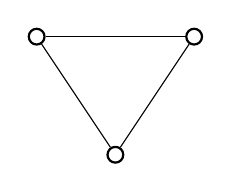
\begin{tikzpicture}[
        mass/.style = {draw,circle, minimum size=0.2cm, inner sep=0pt, thick},
        spring/.style = {decorate,decoration={zigzag, pre length=1cm,post length=1cm,segment length=5pt}},]
        \node[mass] (m1) at (1,1.5) {};
        \node[mass] (m2) at (-1,1.5) {};
        \node[mass] (m3) at (0,0) {};

        \draw (m1) -- (m2);
        \draw (m1) -- (m3);
        \draw (m2) -- (m3);
    \end{tikzpicture}
    \caption{A simple graph with three vertices and three edges}
\end{figure}
\begin{definition}
    A $\Lambda$-decorated graph is given by an ordered pair $(\Gamma,
    \Lambda)$ of a finite graph $\Gamma$ and a set of positive integers
    $\Lambda$ with the labeling
    \begin{itemize}
        \item of the vetices $v\in \Gamma ^{(0)}$ given by $n(\nu) \in
            \Lambda$
        \item of the edges $e = (\nu _1, \nu _2) \in \Gamma ^{(1)}$ by
            operators
            \begin{itemize}
                \item $D_e: \mathbb{C}^{n(\nu _1)} \rightarrow
                    \mathbb{C}^{n(\nu _2)}$
                \item and $D_e^*: \mathbb{C}^{n(\nu _2)} \rightarrow
                    \mathbb{C}^{n(\nu _1)}$ its conjugate traspose
                    (pullback?)
            \end{itemize}
    \end{itemize}
    such that
    \begin{equation}
        n(\Gamma ^{(0)}) = \Lambda
    \end{equation}
\end{definition}
\begin{question}
    Would then $D_e$ be the pullback?
\end{question}
\begin{question}
    These graphs are important in the next chapter I should look
    into it more, I don't understand much here, specific
    how to construct them with the abstraction of a spectral triple...
\end{question}

The operator $D_e$ between $\textbf{n}_i$ and $\textbf{n}_j$ add up to
$D_{ij}$
\begin{align*}
    D_{ij} = \sum\limits_{\substack{e = (\nu _1, \nu _2) \\ n(\nu _1) =
    \textbf{n}_i \\ n(\nu _2) = \textbf{n}_j}} D_e
\end{align*}

\begin{theorem}
    There is a on to one correspondence between finite spectral triples
    modulo unitary equivalence and $\Lambda$-decorated graphs, given by
    associating a finite spectral triples $(A, H, D)$ to  a $\Lambda$ decorated
    graph $(\Gamma, \Lambda)$ in the following way:
    \begin{equation}
        A = \bigoplus _{n\in \Lambda} M_n(\mathbb{C}); \;\;\;
        H = \bigoplus _{\nu \in \Gamma ^{(0)}} \mathbb{C}^{n(\nu)}; \;\;\;
        D = \sum _{e \in \Gamma ^{(1)}} D_e + D_e^*
    \end{equation}
\end{theorem}
\begin{example}
\begin{figure}[h!]
    \centering
    \begin{tikzpicture}[
        mass/.style = {draw,circle, minimum size=0.3cm, inner sep=0pt, thick},
    ]

    \node[mass, label={\textbf{n}}] (m1) at (1,0) {};
    \draw (m1) to [out=330, in=210, looseness=25] node[above] {$D_e$} (m1);
    \end{tikzpicture}
    \caption{A $\Lambda$-decorated Graph of $(M_n(\mathbb{C}), \mathbb{C}^n,
    D = D_e + D_e^*)$}
\end{figure}
\end{example}
\end{document}
